\chapter{ndnSIM}

NDN is a newly proposed Internet communication paradigm that tries to keep most of the well accepted and tested TCP/IP Internet architecture while evolving the thin waist introducing many new features. These features differ in fundamental ways from a point-to-point communication architecture and need to be simulated extensively under ever changing parameters and implementations.

ndnSIM is an open source simulator for NDN networks within the existing NS-3 simulator framework. It's main goals are to facilitate experimentation inside the research community and make all basic NDN protocol operations accessible and therefore changeable like routing, data caching, packet forwarding and congestion management. Packet-level interoperability with CCNx implementation is given in order to support traffic measurements, traffic traces and analysis tools between CCNx and ndnSIM. Large-scale simulations should be supported and made easy to set up through helper classes. Helper classes automate the repetitive creation of single entities like nodes and set them up in a standardized way. Therefore the simulator has been implemented in a very modular fashion making it very easy to modify or replace or re-implement specific components like the FIB , PIT or forwarding strategy. Replacing components have no or minimal impact on other components as long as they adhere to the modules API's and other components they interact with.

\section{Design overview}

NS-3 and ndnSIM both follow a philosophy of maximum abstraction for all modeled components making experimentation on one hand very fine-grained and on the other hand very isolated and decoupled from the rest. The NDN core protocol stack can be installed on every simulated network node in a consistent manner through helpers that take care of all the parts that need to play together like the inter-node communication with installed applications through their respective application faces.

\begin{figure}[H]
  \centering
  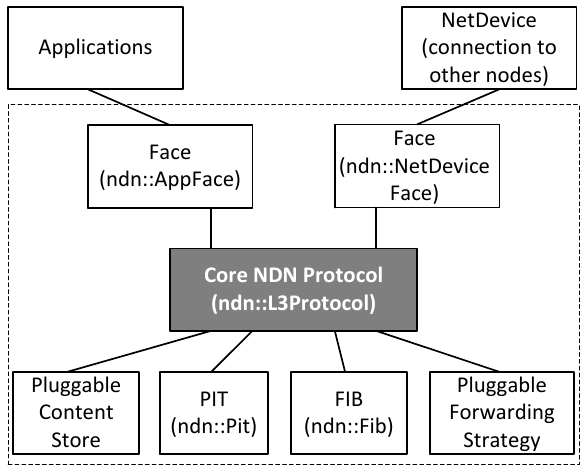
\includegraphics[scale=0.4]{chapter-3/ndnSIMcomponentAbstraction}
  \caption{Basic component abstractions in ndnSIM}
  \label{fig:ndnSIMcomponentAbstraction}
\end{figure}

The basic component abstractions are seen in figure \ref{fig:ndnSIMcomponentAbstraction}. The core NDN Protocol is the ndn::L3Protocol that receives interest and data packages from upper and lower layers through the corresponding faces. As of ndnSIM version 2.0 there are two distinct faces. The application face (ndn::AppFace) is responsible for inter-node communication between the application and the node itself while the net device face (ndn::NetDeviceFace) is responsible for inter-network communication with different nodes. Other faces for different purposes are expected to be added by the core developer or the community as needed. The ndn::ContentStore is an abstraction for in-network caching of data and can easily be omitted or replaced by another implementation of a different storing policy. The ndn::Pit abstracts the data structure that is responsible to log all received interests with their nonce and incoming faces while the FIB abstracts the data structure to guide the strategy in interest forwarding. The ndn::ForwadingStrategy is responsible to implement how interests and data are forwarded. That includes lookups in the content store for cached data, in PIT for already forwarded interests and in FIB if both previous searches didn't yield any matches. Each step is represented as virtual function calls in the forwarder header class of ndnSIM and can be overwritten.

\subsection{Face abstraction}

The face abstraction plays an important role in the overall modularity of the NDN simulator by acting as an interface therefore making ndnSIM design independent from any underlying transport layers. All communication between application and the NDN core protocol and other nodes with the L3 protocol happens through faces that take care of any needed conversion.

\begin{figure}[H]
  \centering
  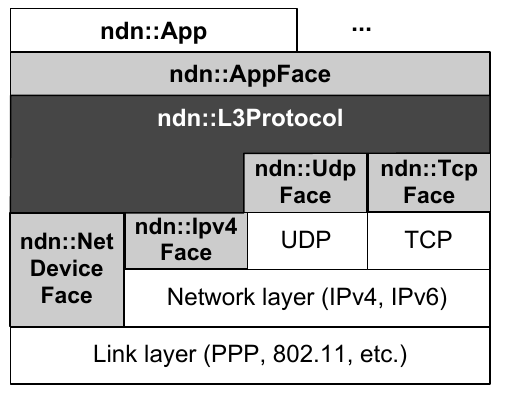
\includegraphics[scale=0.4]{chapter-3/CommunicationLayerAbstraction}
  \caption{Face abstractions around ndn::l3Protocol}
  \label{fig:CommunicationLayerAbstraction}
\end{figure}

As shown in \ref{fig:CommunicationLayerAbstraction} the application can communicate with ndn::L3Protocol through the AppFace whereas for inter-node transmission it depends on the transmission protocols which faces need to be used. TCP and UDP have their respective ndn::UdpFace and ndn::TcpFace. IPv4 and IPv6 also have their own ndn::Ipv4Face making it particularly easy to implement the NDN architecture on top of IP or even TCP/IP. If NDN needs to be implemented without TCP/IP protocol it can communicate directly with the link layer through the ndn::NetDeviceFace.

\subsection{Content Store abstraction}

The CS is crucial for the NDN Internet architecture as it caches data for later use in potentially all the intermediate nodes. It can do rudimentary error recovery and multicast the data asynchronously downstream to the requesters. The replacement policy does determin what data is saved into cache and how it gets replaced or deleted after a certain time. Currently implemented versions of the CS support Leas Recently Used (ndn::cs::Lru), First In First Out (ndn::cs::Fifo) and a Random Replacement Policy (ndn::cs::Random). Each implementation is based on a dynamic trie-based data structure with hash-based indexing as are the PIT and FIB implementations.

\subsection{Pending Interest Table (PIT) abstraction}

The PIT data structure keeps information about each forwarded interest. Each PIT entry is uniquely identified by the content name of the interest. It holds a list of all incoming faces on which the interest was received and a list of all outgoing faces the interest has been forwarded to. The arrival and expiration time are also kept in order to retransmit a lost interest. The nonce of an interest is a randomly generated number that is attached to the interest and identifies the interest for loop detection. Different consumers issuing the same interest will very likely have different nonces. In that case no loop is detected and the incoming face is added to the already existing PIT entry.

\begin{figure}[H]
  \centering
  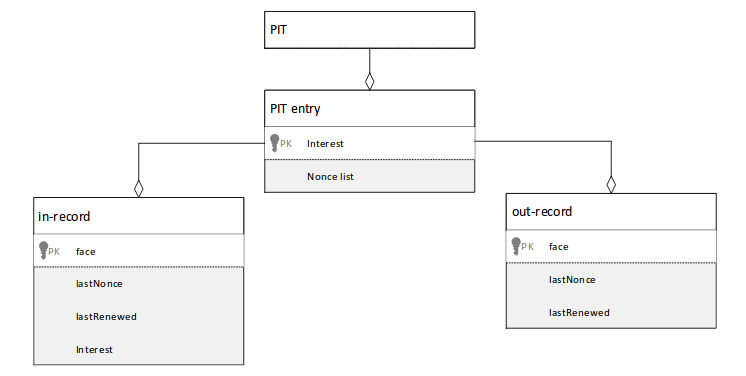
\includegraphics[scale=0.4]{chapter-3/PITdataStructure}
  \caption{PIT data structure}
  \label{fig:PITdataStructure}
\end{figure}

Figure \ref{fig:PITdataStructure} shows the different PIT classes and how they relate to each other. There are also two additional timers on every PIT entry that are not explicitly shown here. The \emph{unsatisfy timer} is the lifetime of an interest and counts down. If it reaches 0 the PIT entry has expired and needs to be forwarded again. The \emph{straggler timer} starts counting down as soon a interest got rejected or satisfied. The straggler timer gives the node the time to detect further loops by the satisfied or rejected interest still floating within the network. Also measurements might require to still finish just after that event. After the straggler timer runs out the PIT entry is deleted. The PIT abstraction provides basic functions to insert, lookup, delete and get measurements.

\subsection{Forwarding Information Base (FIB) abstraction}

The FIB guides the forwarding strategy in making decisions about Interest forwarding. It is similar to an IP's FIB but contains name prefixes instead of IP prefixes and holds several interfaces (out-faces) therefore enabling multicast forwarding. The faces are ordered according to their cost (routing metric) putting the cheapest connections at the beginning of the list. The lookup is performed on the content name prefixes. The longest prefix match yields the requested FIB entry with it's outgoing face(es).

\begin{figure}[H]
  \centering
  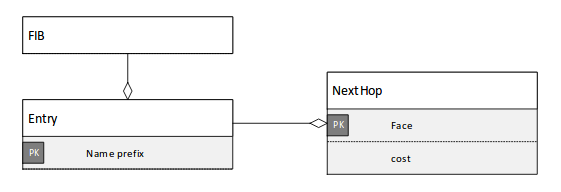
\includegraphics[scale=0.4]{chapter-3/FIBdataStructure}
  \caption{FIB data structure}
  \label{fig:FIBdataStructure}
\end{figure}

As shown in Figure \ref{fig:FIBdataStructure} each FIB entry that has been identified by longest-prefix match has an aggregated collection of NextHops. The NextHop collection must be non-empty and for every NextHop there is one outgoing face toward a possible content source. There may only be one NextHop with a specific face id. The FIB abstraction provides basic insertions, deletions and exact match operations.

\subsection{Forwarding Strategy abstraction}

ndnSIM's modular architecture allows to experiment with different types of forwarding strategies without having to adapt any core components. The forwarder class interacts with the strategy and has the following important functions:

\begin{itemize}
\item \emph{onIncomingInterest}: checks for localhost violations and if the interests has looped. It then inserts or updates the pit, resets it's timers and looks if the interest can be satisfied by cached data.
\item \emph{onContenStoreMiss}: if there is no data to satisfy the interest, the strategy is called.
\item \emph{onOutgoingInterest}: this function is called by the strategy and forwards the interest to the outgoing faces.
\item \emph{onIncomingData}: checks for localhost violations and if there are any PIT entries for that data. If there are no PIT entries the data is dropped, otherwise the data will be handed on to the onOutgoingData function.
\item \emph{onOutgoingData}: forwards the data downstream towards the content requester.
\end{itemize}


The strategy is called on three occasions. The first time from the forwarder::onContentStoreMiss() when the decision has to be made how to forward the interest upstream. A second time from the forwarder::onContentStoreHit() to decide how to proceed with an satisfied interest. And a last time from the forwarder::onIncomingData()

\vspace{5mm} %5mm vertical space

The strategy has one important function:

\begin{itemize}
\item \emph{afterReceiveInterest}: it receives the interest and the corresponding FIB and PIT entries from the forwarder and decides how to forward them further and through which faces.
\end{itemize}

\section{Simulation Environment}

The NS-3 simulator supports several simulation environments. In this theses NS-3 PyViz was used as a live simulator. PyViz also has an interactive console that vizualizes the connections between the nodes of the simulation. It also can be used to degub the state of the running object, show PIT and FIB entries in live and where packages are being dropped.

\begin{figure}[H]
  \centering
  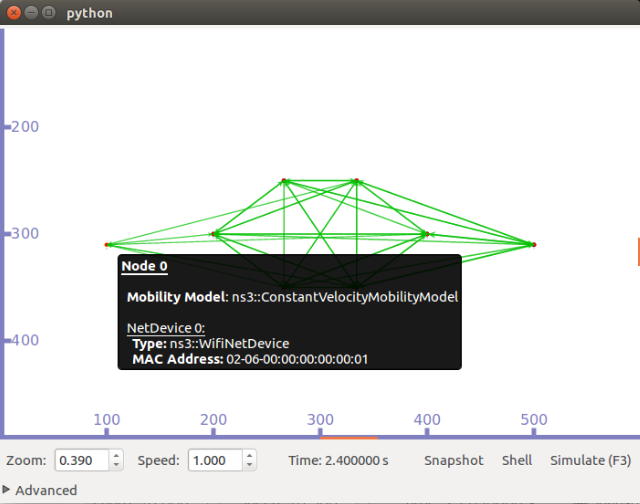
\includegraphics[scale=0.4]{chapter-3/Simulation}
  \caption{Simulation of a possible scenario}
  \label{fig:Simulation}
\end{figure}

Figure \ref{fig:Simulation} shows a current scenario in development. Zoom and speed can interactively be set, the simulation started and paused at any time. Node specific information can be shown while hovering over the node.

\begin{figure}[H]
  \centering
  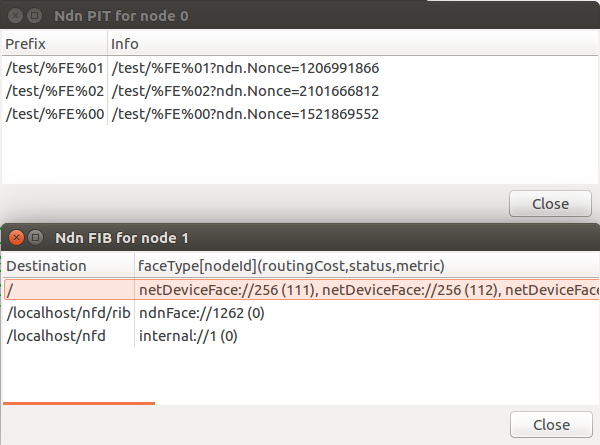
\includegraphics[scale=0.4]{chapter-3/PITandFIBvis}
  \caption{PIT and FIB entries in real time}
  \label{fig:PITandFIBvis}
\end{figure}

Figure \ref{fig:PITandFIBvis} shows all the PIT and FIB entries in real time. Face id's with the corresponding face type are also shown for easier debugging purposes.